\chapter{Quick Intro}

\section{Simple Network Scenario}
\label{sec:SimpleNetworkScenario}
In this section we will show how to build, configure and simulate the following
simple network topology:

Personal computers (\emph{office-pc1} and \emph{office-pc2}) from the network
192.168.1.0/24 are connected to the LAN switch (\emph{office-switch}) which is
connected to the router (\emph{office-router}). The server (\emph{office-host})
from the network 192.168.2.0/24 is directly connected to the router
(\emph{office-router}). Personal computers from the first network have route
only to the network 192.168.2.0/24. The server from the second network has the
default route. Quagga routing is enabled on the router in order to be able to
serve and receive dynamic route updates.

\subsection{Building a simple network}
After running IMUNES on FreeBSD with some kind of X11 window manager (see
Section \ref{sec:UserInterfaceLayout}), we will build previously described
network using tools from the toolbox (see Section \ref{sec:toolbox}).

\subsubsection{Adding and deleting network elements}
To draw a node click on the corresponding node tool and then click on the
workspace to place it. To connect nodes click on the \emph{Link tool}, then
click and hold on the source node and go to the destination node.

Now draw a router, a host, a LAN switch and two PCs. Using the \emph{Link tool}
connect the LAN switch to the router and then connect each PC to the LAN
switch. Connect the host directly to the router. The created network topology
should look like the one in Figure \ref{fig:simple_topology}.

\begin{figure}[H]
\centering
\vspace{10pt}
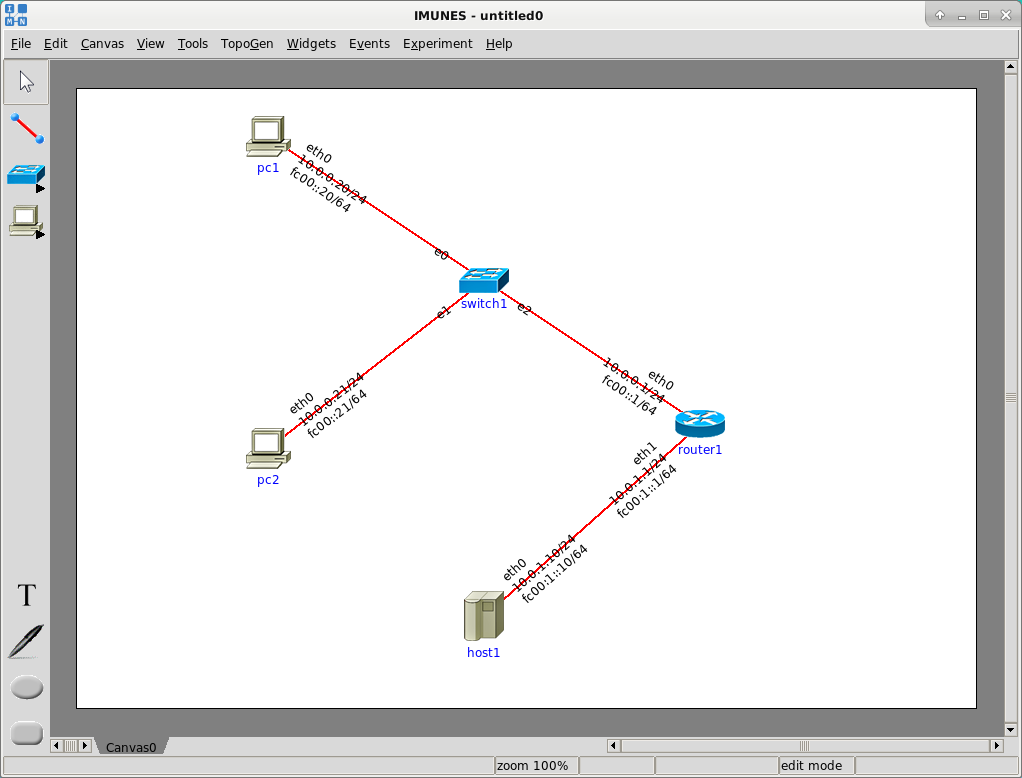
\includegraphics[width=\textwidth]{./images/simple_topology.png}
\caption{\emph{Simple network topology}}
\label{fig:simple_topology}
\end{figure}

When nodes are connected with the \emph{Link tool} (the direction does not
matter), the source node, the destination node and the link automatically get
preconfigured parameters. When a mouse pointer is above a node or a link, some
of the configured parameters are shown on the left side of the statusbar placed
at the bottom of the window (Figure \ref{fig:statusbar_node}).

\begin{figure}[H]
\centering
\vspace{10pt}
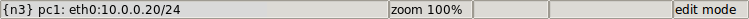
\includegraphics[width=\textwidth]{./images/statusbar1.png}
\caption{\emph{Node parameters in the statusbar}}
\label{fig:statusbar_node}
\end{figure}

Some of the parameters can be visible on the canvas: interface names (link
layer: e0, e1, e2 and network layer: eth0, eth1), IPv4/IPv6 addresses of
network layer elements (PC, host, router), node names (router1, host1, switch1,
pc1, pc2) and link labels (Bandwidth, Delay, BER or Duplicate if their values
are not default).

You can manipulate with the visibility of nodes and links parameters from the
View menu (Figure \ref{fig:view_menu1}). In this simple scenario we do not want
for IPv6 addresses to be visible, so we will turn the \emph{Show IPv6
Addresses} option off.

\begin{figure}[H]
\centering
\vspace{10pt}
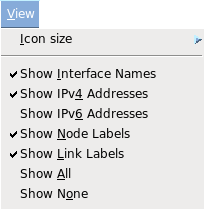
\includegraphics[width=0.28\textwidth]{./images/view_menu1.png}
\caption{\emph{Show or hide nodes and links parameters}}
\label{fig:view_menu1}
\end{figure}

To delete the network element select it using the \emph{Select tool} and then
use the \emph{Delete} keyboard button. You can also delete it by right clicking
on it and clicking on the \emph{Delete} label in the popped up menu. The node
deletion is automatically followed by the deletion of associated links.

\subsubsection{Rearranging network elements}
You can change position of the network element (node or link) and/or the node
name. To move both the network element and its name select the network element
with the \emph{Select tool} and drag it to the designated position. To move
only the node name select it with the \emph{Select tool} and drag it to the
designated position.

Using the \emph{Select tool} you can also move around a group of connected
nodes which can be selected using the \emph{Ctrl} keyboard button in addition
to the left click. To select the whole network topology use \emph{Select All}
option from the \emph{Edit} menu.

For automatic rearranging of all network elements or rearranging the selected
group of network elements use \emph{Rearrange} and \emph{Rearrange All} options
from the \emph{Tools} menu. To stop the rearranging process click with the
\emph{Select tool}.

\subsection{Configuring a simple network}

Although preconfigured parameters of network elements are usually sufficient to
start a simulation (automatically provided IPv4/IPv6 addresses, the default
static route on the PC and the host and routing model and protocols parameters
on the router as well), in this scenario we will set up our own parameters.

To open the network element configuration window:
\begin{itemize}
  \item right click on the network element and select the \emph{Configure}
label from the popped up menu (Figure \ref{fig:configure_label}) 
  
  or
  
  \item double click on the network element.
\end{itemize}

\begin{figure}[H]
\centering
\vspace{10pt}
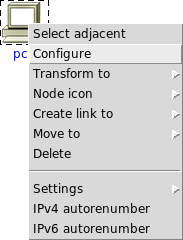
\includegraphics[width=0.28\textwidth]{./images/configure_label.png}
\caption{\emph{Configure a network element}}
\label{fig:configure_label}
\end{figure}

Network elements configuration parameters can be also changed through the
topology tree. To show the topology tree turn on the \emph{Show Topology Tree}
option from the \emph{View} menu. The tree with a list of network topology
elements (nodes and links) will be shown on the right side of the window
(Figure \ref{fig:topology_tree}). To open the network element configuration
window double click or use the \emph{Enter} keyboard button on node, interface
or link label in the topology tree.

\begin{figure}[H]
\centering
\vspace{10pt}
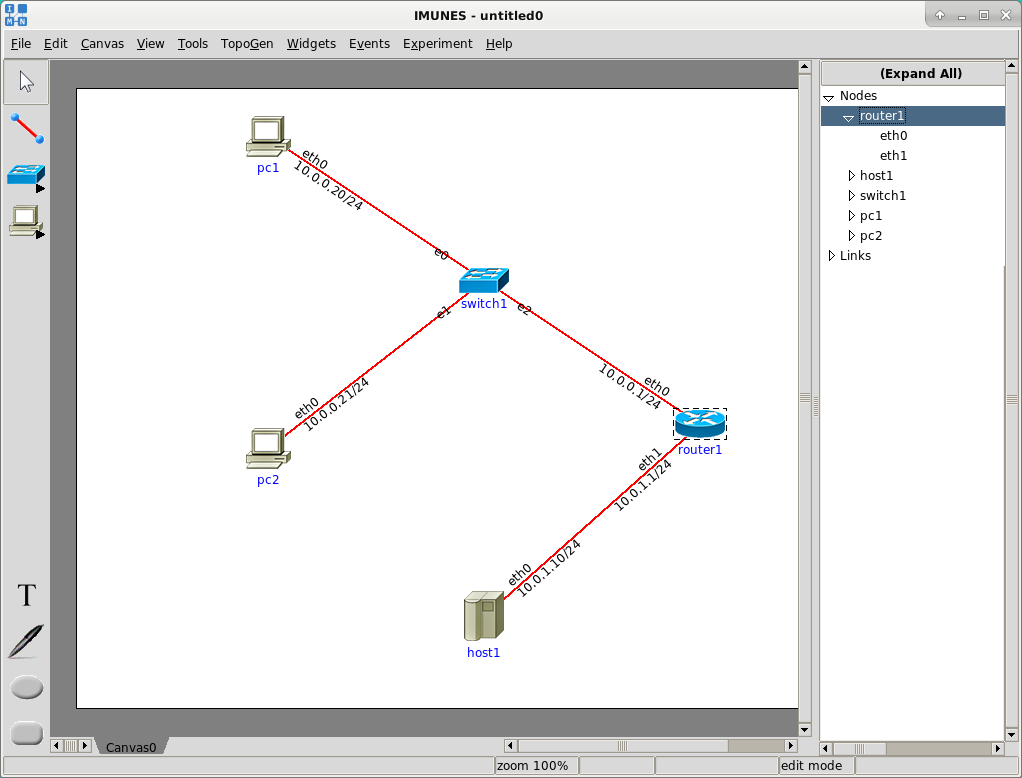
\includegraphics[width=\textwidth]{./images/topology_tree.png}
\caption{\emph{Changing configuration parameters through the topology tree}}
\label{fig:topology_tree}
\end{figure}

Depending on the type of a network element in our topology, there are 4 types
of configuration windows:

\begin{itemize}
  \item \emph{Hub/LAN switch configuration} window
  \item \emph{PC/Host/Click router configuration} window
  \item \emph{Router configuration} window
  \item \emph{Link configuration} window
\end{itemize}

There are also other types of configuration windows which are explained in
other sections:

\begin{itemize}
  \item \emph{External interface configuration} window
  \item \emph{External connection configuration} window
  \item \emph{NAT64 configuration} window
  \item \emph{RSTP switch configuration} window
  \item \emph{Filter node configuration} window
  \item \emph{Packet generator configuration} window
  \item \emph{Click switch configuration} window
\end{itemize}

\subsubsection{Hub/LAN switch configuration window}
The \emph{hub/LAN switch configuration} window, as well as the configuration
windows of other node types, contains a node name field. Besides that it
contains only link layer interface parameters.

We will change the LAN switch name and data packet scheduling method (from
preconfigured First In First Out (FIFO) data packet scheduling method to
Weighted Fair Queuing (WFQ) method).

Change the node name to \emph{office-switch}.
To change data packet scheduling method select the link layer interface
\emph{e0} from the list of interfaces, choose \emph{WFQ} option from the
\emph{Queue} menu and click on the \emph{Apply} button (Figure
\ref{fig:LANswitch_config}). 

\begin{figure}[H]
\centering
\vspace{10pt}
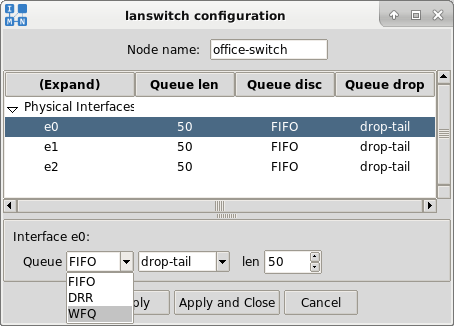
\includegraphics[width=0.6\textwidth]{./images/LANswitch_config.png}
\caption{\emph{LAN switch configuration window}}
\label{fig:LANswitch_config}
\end{figure}

Packet scheduling method is now applied and you can see new queuing discipline
for interface \emph{e0} in the column \emph{Queue disc} (Figure
\ref{fig:LANswitch_config_applied}). 

\begin{figure}[H]
\centering
\vspace{10pt}
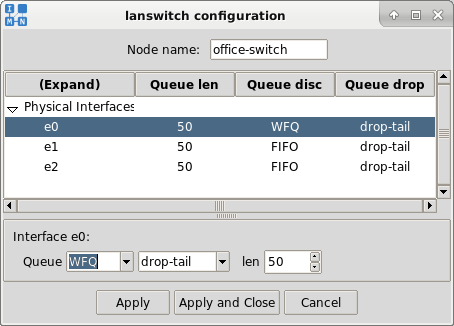
\includegraphics[width=0.6\textwidth]{./images/LANswitch_config_applied.png}
\caption{\emph{LAN switch configuration window with applied changes}}
\label{fig:LANswitch_config_applied}
\end{figure}

Repeat the same procedure for the other link layer interfaces.
Changed configuration is already applied so you can close the configuration
window with the \emph{Cancel} button but you can also use the \emph{Apply and
Close} button.

\subsubsection{PC/Host/Click router configuration window}
The \emph{PC/Host/Click router configuration} window consists of two
subwindows. Each of them is associated with one of the following tabs:
\emph{Configuration} and \emph{Interfaces} (Figure \ref{fig:pc_config_tabs}).

\begin{figure}[H]
\centering
\vspace{10pt}
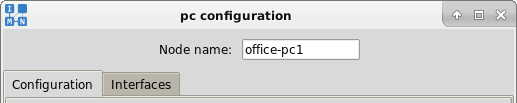
\includegraphics[width=0.6\textwidth]{./images/pc_config_tabs.png}
\caption{\emph{Tabs in the PC/Host/Click router configuration window}}
\label{fig:pc_config_tabs}
\end{figure}

Besides a node name field, \emph{PC/Host/Click router configuration} window
contains startup services, routing parameters and custom configuration
parameters (in the window associated with the \emph{Configuration} tab) and
network interface parameters (in the window associated with the
\emph{Interfaces} tab).

We will change the node name, network interface parameters and routing
parameters.

Change the host node name to \emph{office-host} and PC node names to
\emph{office-pc1} and \emph{office-pc2}.
To change IPv4 address left click on the \emph{Interfaces} tab, select
interface \emph{eth0} from the list of interfaces, change the IPv4 address
field and click on the \emph{Apply} button (Figure \ref{fig:pc_config_ipv4}).
We will change the host IPv4 address field to 192.168.2.5/24 (now it belongs to
192.168.2.0/24) and PC IPv4 address fields to 192.168.1.5/24 and 192.168.1.7/24
(now they belong to network 192.168.1.0/24). IP address fields require the CIDR
notation, so the IPv4 address is followed by a slash and a network length.

\begin{figure}[H]
\centering
\vspace{10pt}
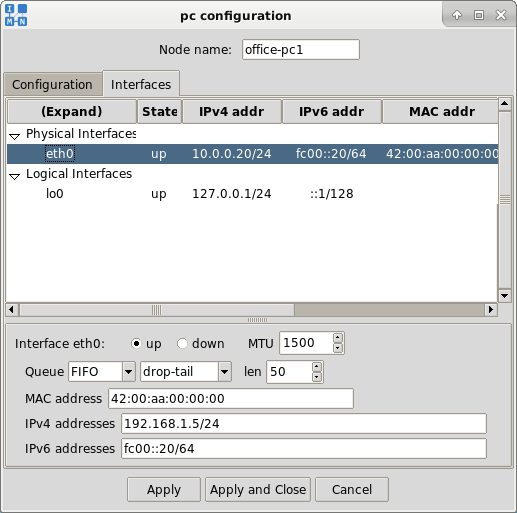
\includegraphics[width=0.6\textwidth]{./images/pc_config_ipv4.png}
\caption{\emph{Changing IPv4 address}}
\label{fig:pc_config_ipv4}
\end{figure}

\paragraph{\emph{Static routes}} \hfill

PCs and Hosts both use static routing. The preconfigured routing table contains
only the default route. Every static route, as well as the default route,
consists of:
\begin{enumerate}
  \item the destination network: an IP address which is followed by a slash and
a network prefix and
  \item the next hop network interface IP address (which is an IP address
without a slash and without a network prefix).
\end{enumerate}

If the route syntax is wrong, that route will be silently ignored. 

We will add the static route on \emph{office-pc1} and \emph{office-pc2} for the
network 192.168.2.0/24 through the gateway 192.168.1.1 (Figure
\ref{fig:pc_config_staticroutes}). 

\begin{figure}[H]
\centering
\vspace{10pt}
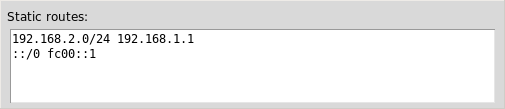
\includegraphics[width=0.6\textwidth]{./images/pc_config_staticroutes.png}
\caption{\emph{Adding the static route on the PC}}
\label{fig:pc_config_staticroutes}
\end{figure}

On \emph{office-host} we will change default gateway address to 192.168.2.1
(Figure \ref{fig:host_config_staticroutes}).

\begin{figure}[H]
\centering
\vspace{10pt}
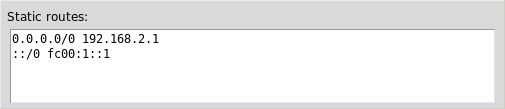
\includegraphics[width=0.6\textwidth]{./images/host_config_staticroutes.png}
\caption{\emph{Adding the static route on the PC}}
\label{fig:host_config_staticroutes}
\end{figure}

IPv6 addresses and default routes (placed below IPv4 addresses and routes) can
be deleted.

To apply the changed configuration and close the configuration window click on
the \emph{Apply and Close} button.

\subsubsection{Router configuration window}
The \emph{router configuration window}, in addition to fields from
\emph{PC/Host/Click router configuration} window, contains the part for
choosing the routing model and protocols, as well as an \emph{IPsec} tab with
IPsec parameters (See IPsec Section TODO).

We will only change the node name and network interface parameters.

Change the node name to \emph{office-router} and IPv4 addresses on both network
interfaces: 192.168.1.1/24 on the network interface \emph{eth0} and
192.168.2.1/24 on the network interface \emph{eth1}.

\paragraph{\emph{Routing models and protocols}} \hfill

There are three possible routing models:
\begin{enumerate}
  \item the quagga model
  \item the xorp model (eXtensible Open Router Platform)
  \item the static model
\end{enumerate}

In the case of quagga and xorp routing models, there are options for
enabling/disabling RIP, RIPng, OSPFv2 and OSPFv3. By default, all new quagga or
xorp router instances will have both RIPv2 and RIPng enabled. The defaults can
be changed with the \emph{Tools $\to$ Routing protocol defaults} option from
the menubar, which will be applied to all selected routers (if any) at the time
of change, as well as to all the subsequentially created ones (see Section
\ref{sec:RoutingProtocolDefaults}).
In the case of static routing model, the router uses routes from the static
routes field that has the same syntax as the static routes field in the
\emph{PC/Host/Click router configuration} window.

We will leave the default router model - quagga with RIP and RIPng protocols
enabled, and OSPFv2 and OSPFv3 protocols disabled (Figure
\ref{fig:router_config_routingmodels}).

\begin{figure}[H]
\centering
\vspace{10pt}
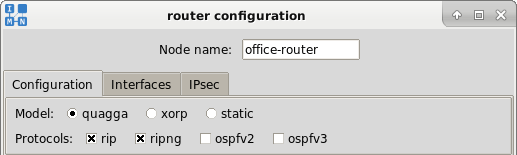
\includegraphics[width=0.6\textwidth]{./images/router_config_routingmodels.png}
\caption{\emph{Routing models and protocols}}
\label{fig:router_config_routingmodels}
\end{figure}

\subsubsection{Link configuration window}
The \emph{link configuration} window offers the possibility to configure the
link bandwidth (between 0 and 10\textsuperscript{9} bps), the propagation delay
(between 0 and 10\textsuperscript{7} $\mu$s), the bit error
rate (between 0 and 10\textsuperscript{12}) and the probability of package
duplication (between 0 and 50\%). There are also display properties: the link
width (line thickness between 1 and 8) and the link color (red, green, blue,
yellow, magenta, cyan or black).

\begin{figure}[H]
\centering
\vspace{10pt}
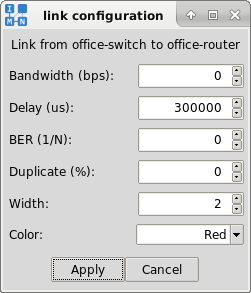
\includegraphics[width=0.4\textwidth]{./images/link_config.png}
\caption{\emph{Link configuration window}}
\label{fig:link_config}
\end{figure}

Default values are as follows: the link which transmits packets without errors
and without any possibility for the packet duplication with the unlimited link
bandwidth and the zero propagation delay. The link width is set to value 2 and
the link color is red.

We will leave default values on all links except on the link between
\emph{office-switch} and \emph{office-router} (Figure
\ref{fig:configured_topology}). On that link we will set up the delay of 30000
$\mu$s. Delay will be tested during the network simulation with the
\emph{traceroute} tool (see Section \ref{sec:NodeandLinkMenuOptions}).

\subsubsection{Configured network topology}
Configured network topology should look like the one in Figure
\ref{fig:configured_topology}.

\begin{figure}[H]
\centering
\vspace{10pt}
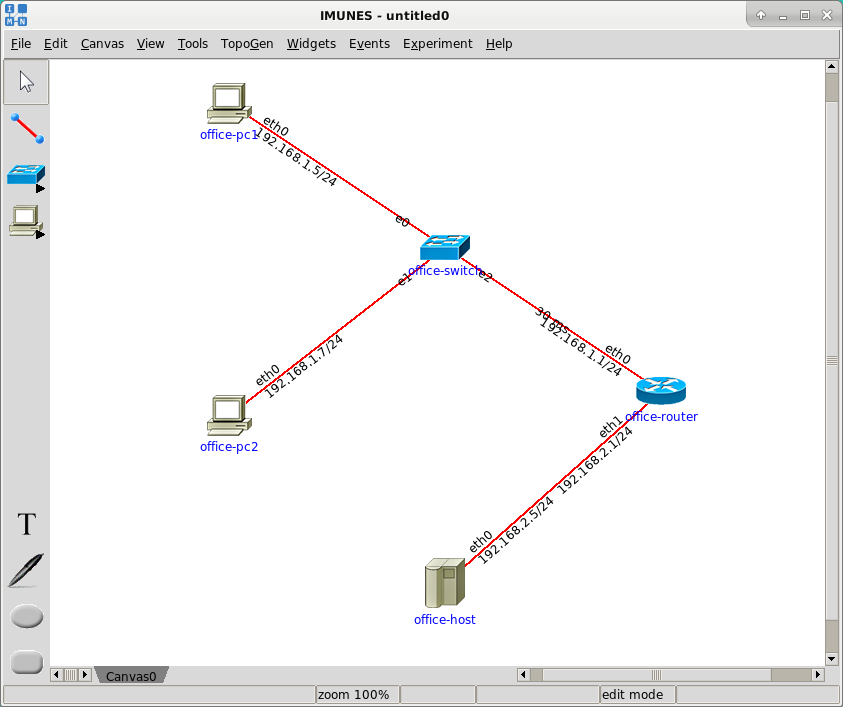
\includegraphics[width=\textwidth]{./images/simple_topology_configured.png}
\caption{\emph{Configured network topology}}
\label{fig:configured_topology}
\end{figure}

\subsection{Simulating a simple network}
\label{sec:simulating a simple network}

\subsubsection{Starting an experiment}
After the network topology is completely built and properly configured, we will
start an experiment with the \emph{Experiment $\to$ Execute}  option from the
menubar and IMUNES will switch from the edit mode to the execute mode. In the
process of starting an experiment, IMUNES creates and configures the virtual
network. That will take a few seconds and all events during that process will
be shown in the statusbar placed at the bottom of the window.

\textbf{NOTE:} Although you can draw network topology on any system that
supports Tcl/Tk (Linux, FreeBSD, Windows, Mac OS X, Solaris), an  experiment
can only be started on FreeBSD and Linux operating systems with root
permissions (Figure \ref{fig:execute_windows} and Figure
\ref{fig:execute_not_root})!

\begin{figure}[H]
\centering
\vspace{10pt}
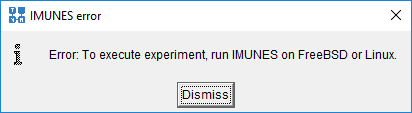
\includegraphics[width=0.7\textwidth]{./images/execute_windows.png}
\caption{\emph{Starting an experiment in Windows}}
\label{fig:execute_windows}
\end{figure}

\begin{figure}[H]
\centering
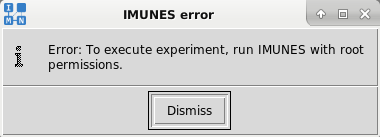
\includegraphics[width=0.5\textwidth]{./images/execute_not_root.png}
\caption{\emph{Starting an experiment in FreeBSD without root permissions}}
\label{fig:execute_not_root}
\end{figure}
 
In addition to configured parameters, each node will be set with the loopback
interface, a router will have the kernel forwarding enabled, and a host node
will have portmap and inetd started.

Information about the time spent instantiating the network topology is shown in
the statusbar (Figure \ref{fig:statusbar_execute}).

\begin{figure}[H]
\centering
\vspace{10pt}
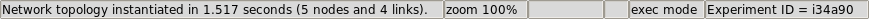
\includegraphics[width=\textwidth]{./images/statusbar3.png}
\caption{\emph{Message about the instantiation of the network topology}}
\label{fig:statusbar_execute}
\end{figure}

In the right corner of the statusbar you can also see that IMUNES now works in
the execute mode, as well as experiment unique identifier.

\subsubsection{Options from the node and the link menu}
\label{sec:NodeandLinkMenuOptions}
To open the node menu in the execute mode right click on the node. Note that
the menu in the execute mode is different from the menu in the edit mode. It
offers the possibility to select the node connected to this node (\emph{Select
adjacent}), to see the current configuration (\emph{Configure}), to \emph{Start
/ Stop / Restart} the network element, to start / stop / restart any of the
possible \emph{Services} or to \emph{Import Running Configuration} from the
\emph{Settings} menu. The \emph{Import Running Configuration} option copies the
current MTU value and IPv4/IPv6 addresses from the running node to its
configuration. It is also possible to open the \emph{Shell window} (X terminal
with a Unix shell), \emph{Wireshark} or \emph{tcpdump} network sniffers on any
of the interfaces, \emph{Firefox} \emph{Web Browser} or a \emph{Mail client}.

\begin{figure}[H]
\centering
\vspace{10pt}
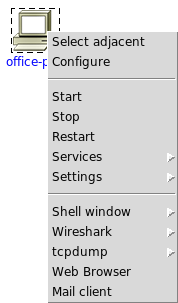
\includegraphics[width=0.28\textwidth]{./images/execute_menu.png}
\caption{\emph{Network-layer node menu in the execute mode}}
\label{fig:execute_menu}
\end{figure}

Note that both the node and the link menu in the execute menu offer the
possibility to open the configuration window (\emph{Configure} label). 

From the node configuration window in the execute mode it is possible to change
only the node name. Other node parameters such as link layer interface
parameters, network interface parameters and routing parameters can be changed
from the shell window on each node. To change those parameters from the node
configuration window, stop the node (using the \emph{Stop} label), change
parameters and then start the node agin (using the \emph{Start} label).

On the other side, from the link configuration window in the execute mode it is
possible to change the following link parameters: link bandwidth, the
propagation delay, the bit error rate and the probability of package
duplication. It is also possible to change display properties: the link
width and the link color.

We will now check if the virtual network topology is properly configured. Open
the shell window (e.g. \emph{Shell window} $\to$ \emph{csh} or simply double
click on the node) on the network element (e.g. \emph{office-pc1}).
\begin{itemize}
\item To check the network interface eth0 parameters type the following
command: \texttt{ifconfig eth0}. The result is shown in Figure
\ref{fig:pc_ifconfig}.

\begin{figure}[H]
\centering
\vspace{10pt}
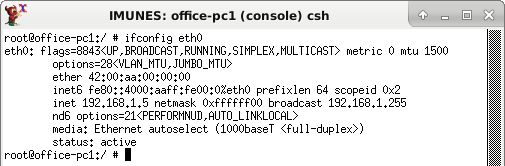
\includegraphics[width=0.8\textwidth]{./images/pc_ifconfig.png}
\caption{\emph{Shell window on office-pc1, network interface parameters}}
\label{fig:pc_ifconfig}
\end{figure}

\item To check static routes type the following command: \texttt{netstat -nrf
inet}. The result is shown in Figure \ref{fig:pc_netstat}.

\begin{figure}[H]
\centering
\vspace{10pt}
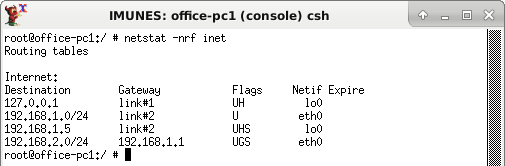
\includegraphics[width=0.8\textwidth]{./images/pc_netstat.png}
\caption{\emph{Shell window on office-pc1, static routes}}
\label{fig:pc_netstat}
\end{figure}

\item To test if a particular network element is reachable (e.g
\emph{office-host}) type the following command: \texttt{ping 192.168.2.5}. The
result is shown in Figure \ref{fig:pc_ping}. To stop transmitting packets press
\emph{Control-C} keyboard button.

\begin{figure}[H]
\centering
\vspace{10pt}
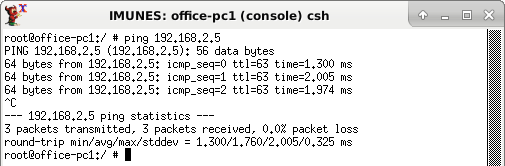
\includegraphics[width=0.8\textwidth]{./images/pc_ping.png}
\caption{\emph{Shell window on office-pc1, pinging office-host}}
\label{fig:pc_ping}
\end{figure}

\end{itemize}

We will test delay on the link between \emph{office-switch} and
\emph{office-router}, which is set to 30000 $\mu$s (30 ms), by using the
\emph{traceroute} tool:
\begin{itemize}
\item In the shell window on \emph{office-pc1} type the following command: \\
\texttt{traceroute 192.168.1.1}. The result is shown in Figure
\ref{fig:pc_traceroute}.

\begin{figure}[H]
\centering
\vspace{10pt}
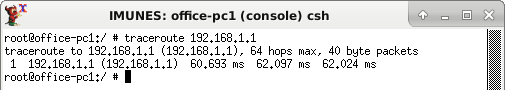
\includegraphics[width=0.8\textwidth]{./images/pc_traceroute.png}
\caption{\emph{Shell window on office-pc1, traceroute to office-router}}
\label{fig:pc_traceroute}
\end{figure}

\item In the shell window on \emph{office-host} type the following command: \\
\texttt{traceroute 192.168.2.1}. The result is shown in Figure
\ref{fig:host_traceroute}.

\begin{figure}[H]
\centering
\vspace{10pt}
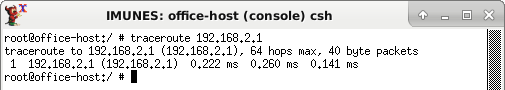
\includegraphics[width=0.8\textwidth]{./images/host_traceroute.png}
\caption{\emph{Shell window on office-host, traceroute to office-router}}
\label{fig:host_traceroute}
\end{figure}

\end{itemize}

\subsubsection{Terminating an experiment}
To terminate an experiment and switch from the execute mode to the edit mode
use the \emph{Experiment $\to$ Execute} option from the menubar. During the
termination process, IMUNES will terminate active services on each node and
shut down all network elements (links and nodes with both virtual and physical
interfaces). The termination is finished when the message about the successful
cleanup shows up in the statusbar (Figure \ref{fig:statusbar4}).

\begin{figure}[H]
\centering
\vspace{10pt}
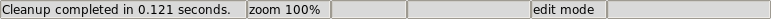
\includegraphics[width=\textwidth]{./images/statusbar4.png}
\caption{\emph{Message about the successful cleanup}}
\label{fig:statusbar4}
\end{figure}

\section{Configuration files management}

\subsection{Saving a virtual network configuration}

After the virtual network is successfully built, configured and tested, it can
be saved with \emph{File $\to$ Save} or \emph{File $\to$ Save As} options from
the menubar. The virtual network topology is saved in IMUNES network
configuration file format (.imn).

\begin{figure}[H]
\centering
\vspace{10pt}
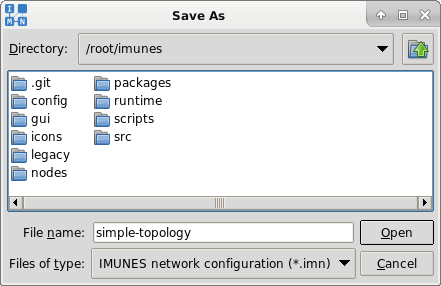
\includegraphics[width=0.65\textwidth]{./images/file_save.png}
\caption{\emph{File Save dialog}}
\label{fig:file_save}
\end{figure}

The structure of the configuration file is simple and suitable for changing
with a text editor (see Appendix \ref{sec:IMUNESNetworkConfigurationFile}).

\subsection{Opening a virtual network configuration}
To open an existing IMUNES network configuration file use the \emph{File $\to$
Open} option from the menubar and select it from the invoked \emph{File Open}
dialog. 

\begin{figure}[H]
\centering
\vspace{10pt}
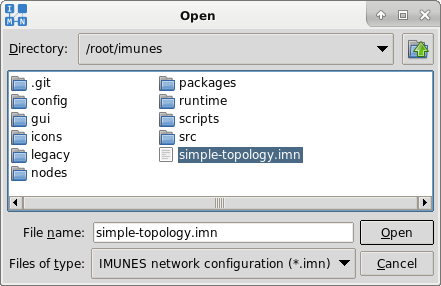
\includegraphics[width=0.65\textwidth]{./images/file_open.png}
\caption{\emph{File Open dialog}}
\label{fig:file_open}
\end{figure}

The other way to open an imn file is to start IMUNES with that file as an
argument: \texttt{imunes simple-topology.imn}
